\chapter{Variables and calculations}
	\label{ch:var}                                                                                                                                                                                                               
	This chapter explains:
	\begin{itemize}
		\item the types of numeric variables;
		\item how to declare variables;
		\item the assignment statement;
		\item arithmetic operators;
		\item the use of numbers with labels and text boxes;
		\item the essentials of strings.
	\end{itemize}

	\section{Introduction}
		Numbers of one type or another occur in most programs, for example, drawing pictures using screen coordinates, controlling spaceflight trajectories, calculating salaries and tax deductions.

		Here we will introduce the two basic types of number:
		\begin{itemize}
			\item whole numbers, known as integers in maths and as the \keyword{Integer} type in VB;
			\item 'decimal-point' numbers, known as 'real' in maths, 'float' in C++ and Java, and as \keyword{Double} in VB. The general term for decimal-point numbers in computing is \emph{floating-point}.
		\end{itemize}
		
		Previously we used values to produce screen graphics, but for more sophisticated programs we need to introduce the concept of a variable – a kind of storage box used to remember values, so that these values can be used or altered later in the program.
		
		There are undeniably some \keyword{Integer} situations:
		\begin{itemize}
			\item the number of students in a class;
			\item the number of pixels on a screen;
			\item the number of copies of this book sold so far; 
		\end{itemize}
			
		and there are some undeniable \keyword{Double} situations:
		\begin{itemize}
			\item my height in metres;
			\item the mass of an atom in grams;
			\item the average of the integers 3 and 4.
		\end{itemize}
		
		However, sometimes the type is not obvious; consider a variable for holding an exam mark – \keyword{Double} or \keyword{Integer}? The answer is that you don't know yet – you must seek further clarification, e.g. by asking the marker if they mark to the nearest whole number, or if they ever use decimal places. Thus, the choice of \keyword{Integer} or \keyword{Double} is determined by the problem.

	\section{The nature of Integer}
		When we use an Integer in VB, it can be a whole number in the range −2147483648 to +2147483647 or, approximately −2000000000 to +2000000000.
		All \keyword{Integer} calculations are accurate, in the sense that all the information in the number is preserved correctly.

	\section{The nature of \keyword{Double}}
		When we use a \keyword{Double} number in VB, its value can be between $−1.79 × 10^{308}$ to $+1.79 × 10^{308}$. In less mathematical terms, the largest value is 179 followed by 306 zeroes – very large indeed! Numbers are held to an approximate accuracy of 15 digits.
		
		The main point about \keyword{Double} quantities is that they are stored approximately in many cases. Try this on a calculator:
		\begin{lstlisting}
7 / 3
		\end{lstlisting}
		Using seven digits, for example, the answer is 2.333333, whereas we know that a closer answer is:
2.33333333333333333
		Even this is not the exact answer!
		
		In short, because \keyword{Double} quantities are stored in a limited number of digits, small errors can build up at the least significant end. For many calculations (e.g. exam marks) this is not important, but for calculations involving, say, the design of a space shuttle, it might be. However, \keyword{Double} has such a large range and digits of precision that calculations involving everyday quantities will be accurate enough.

	\section{Declaring variables}
		Once the type of our variables has been chosen, we need to name them. We can imagine them as storage boxes with a name on the outside and a number (value) inside. The value may change as the program works through its sequence of operations, but the name is fixed. The programmer is free to choose the names, and we recommend choosing meaningful ones rather than cryptic ones. But as in most programming languages, there are certain rules that must be followed. In VB, names:
		\begin{itemize}
			\item must start with a letter (A to Z, a to z);
			\item can contain any number of letters or digits (a digit is 0 to 9);
			\item can contain the underscore '\_';
			\item can be up to 255 characters long.
		\end{itemize}
		Note that VB is not case-sensitive. If a programming language is case-sensitive, we can have two different variables with different capitalization, such as \keyword{width} and \keyword{Width}. In VB, once you have declared \keyword{width}, any attempt to declare a variable \keyword{Width} will result in a compilation error. Your variables must differ in spelling, not just capitalization.
		
		Those are the VB rules – and we have to obey the rules. But there is also a VB style – a way of using the rules which is followed when a variable consists of several words. The rules do not allow spaces in names, so rather than use short names or the underscore, the accepted style for variables is to capitalize the start of each word.
		
		There is another style guideline regarding whether or not the first letter of a name is capitalized. In this chapter we are dealing with variables that are only used within a method (rather than being shared between several methods). Variables such as these are known as \emph{local} and can only be used between the \keyword{Sub} and the \keyword{End Sub} in which they are declared. Returning to style conventions, the VB approach is to \emph{not} capitalize the first letter of local variables. Later, we will see that other types of name, such as method names, control names and class names are conventionally begun with a capital letter.
		
		Thus, rather than:
		\begin{lstlisting}
Heightofbox
h
hob
height_of_box
		\end{lstlisting}
		we put:
		\begin{lstlisting}
heightOfBox
		\end{lstlisting}
		Here are some allowed names:
		\begin{lstlisting}
amount
x
pay2003
		\end{lstlisting}
		and here are some unallowable (illegal) names:
		\begin{lstlisting}
2001pay
_area
my age
		\end{lstlisting}
		Note that there are also some reserved names that VB uses and which cannott be reused by the programmer. They are termed \emph{keywords} in VB. You have seen some of them, e.g.:
		\begin{lstlisting}
Private
Dim
New
		\end{lstlisting}
A full list is provided in \textcolor{red}{Appendix B}.

		\begin{stqb}
			\begin{STQ}
			\item	Which of the following local variable names are allowed in VB, and which have the correct style?
				\begin{lstlisting}
volume
AREA
Length
3sides
side1	
lenth	
Mysalary
your salary
screenSize
Dim
				\end{lstlisting}
			\end{STQ}
		\end{stqb}

		Here is an example program, named 'Area Rectangle', which we will study in detail. It calculates the area of a rectangle. We have assumed that its sides are \keyword{Integer} quantities. There is only one control on the form – a button with its \keyword{Text} property set to 'Calculate'. All our added code will be inside the \keyword{Button1\_Click} method.
		\begin{lstlisting}
Private Sub Button1_Click( 
	sender As System.Object, 
	e As System.EventArgs) Handles Button1.Click
	Dim area As Integer
	Dim length As Integer
	Dim breadth As Integer
	length = 20
	breadth = 10
	area = length * breadth
	MessageBox.Show("Area is: " & CStr(area))
End Sub
		\end{lstlisting}
		\begin{figure}[ht]
			\centering
			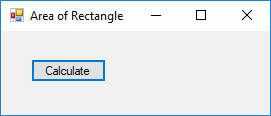
\includegraphics[width=8cm]{var_calc_area}
			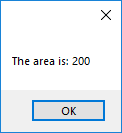
\includegraphics[width=4cm]{var_calc_area_result}
			\caption{Screenshot of Area of Rectangle.}
			\label{fig:var_calc_area}
		\end{figure}

		\Vref{fig:var_calc_area} shows what you will see on the screen.

		In the program we have used three \keyword{Integer} variables, which eventually will hold our rectangle data. Recall that we can choose whatever names we like, but have opted for clear names rather than single-letter or funny names. (Funny names are only funny the first time you see them!)
		Now that names are chosen, we must declare them to the VB system. Though this seems like tedious red tape at first, the point of introducing them is to enable the compiler to spot misspellings lower down the program. Here are the declarations:
		\begin{lstlisting}
Dim area As Integer
Dim length As Integer
Dim breadth As Integer
		\end{lstlisting}
		The word \keyword{Dim} is used to declare local variables that are only going to be used inside one method of the program, between \keyword{Private Sub}, and \keyword{End Sub}. Here our variables are used between \keyword{Sub Button1\_Click} and its matching \keyword{End Sub}. \keyword{Dim} is not a very meaningful name, but it has been carried through from early versions of Basic, where it was short for 'dimension'.
Note the use of \keyword{Integer} to show that each variable will hold a whole number. Alternatively, we could have put:
		\begin{lstlisting}
Dim length, breadth, area As Integer
		\end{lstlisting}
		using commas to separate each name. The style is up to you, but we have a preference for the first style, which enables you to comment each name if you need to. If you use the second style, use it to group related names. For example, put:
		\begin{lstlisting}
Dim pictureHeight, pictureWidth As Integer
Dim myAge As Integer
		\end{lstlisting}
		rather than:
		\begin{lstlisting}
Dim pictureHeight, pictureWidth, myAge As Integer
		\end{lstlisting}
		In the majority of programs we will use several types, and in VB we are free to intermingle the declarations, as in:
		\begin{lstlisting}
Dim personHeight As Double
Dim examMark As Integer
Dim salary As Double
		\end{lstlisting}
Additionally, we can choose to initialize the value of the variable as we declare it, as in:
		\begin{lstlisting}
Dim personHeight As Double = 1.68
Dim a As Integer = 3, b As Integer = 4
Dim examMark As Integer = 65
Dim betterMark As Integer = examMark + 10
		\end{lstlisting}
		This is good style, but only use it when you really know the initial value. If you don't supply an initial value, VB sets numeric variables to zero, and string variables to an empty string.

	\section{The assignment statement}
		Once we have declared our variables, we can place new values in them by means of the 'assignment statement', as in:
length = 20
Pictorially, we can imagine the process as in \Vref{fig:var_assignment}. We say: 'the value 20 has been assigned to the variable \keyword{length}' or '\keyword{length} becomes 20'.
Note:
		\begin{itemize}
			\item The movement of data is from the right of the = to the left.
			\item Whatever value was in \keyword{length} before is now 'overwritten' by 20. Variables have only one value – the current one. And just to give you a flavour of the speed: an assignment takes less than one-millionth of a second.
		\end{itemize}

	\section{Calculations and operators}
		Recall our rectangle program, which included the statement:
		\begin{lstlisting}
area = length * breadth
		\end{lstlisting}

		\begin{figure}[ht]
			\centering
			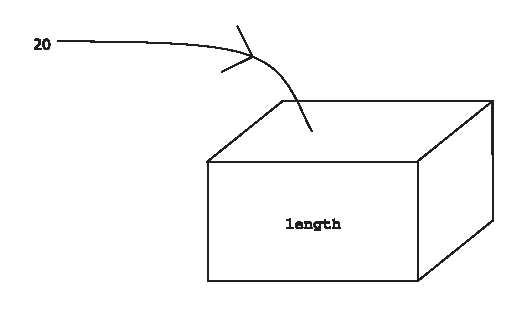
\includegraphics[width=9cm]{var_assignment}
			\caption{Assigning a value to a variable.}
			\label{fig:var_assignment}
		\end{figure}

		The general form of the assignment statement is:
		\begin{lstlisting}
variable = expression
		\end{lstlisting}
		An expression can take several forms: for example, a single number or a calculation. In our specific example, the sequence of events is:
		\begin{enumerate}
			\item '*' causes multiplication of the values stored in \keyword{length} and \keyword{breadth}, resulting in the value 200.
			\item The equals symbol = causes the 200 to be assigned to (stored in) \keyword{area}.
		\end{enumerate}
		The * is one of several 'operators' (so called because they operate on values) and, just as in maths, there are rules for their use.
		
		An understanding of the movement of data is important, and enables us to understand the meaning of code such as:
		\begin{lstlisting}
Dim n As Integer = 10
n = n + 1
		\end{lstlisting}
		What happens is that the right-hand side of the = is calculated using the current value of n, resulting in 11. This value is then stored in n, replacing the old value of 10. In fact, years ago a large number of programs were studied, and statements of the form:
		\begin{lstlisting}
something = something + 1
		\end{lstlisting}
		were found to be the most common instructions!
		
		The conclusion you can draw from the above is that = does not mean 'is equal to' in the algebra sense. You should imagine it as meaning 'becomes' or 'gets'.
	\section{The arithmetic operators}
		Here we present a basic set of operators – the arithmetic ones, akin to the buttons on your calculator. By the way, in this context, we pronounce the adjective 'arithmetic' as 'arithMETic'.

		\begin{center}
			\begin{tabular}{lll}
				\toprule Operator & Meaning\\ \midrule
				\textasciicircum & exponent (power of)\\ \midrule
				$*$ & multiply\\
				$ / $ & division of doubles\\
				$ \backslash $ & division of integers\\
				\keyword{Mod} & modulo\\ \midrule
				+ & add\\
				$-$ & subtract\\ \bottomrule
			\end{tabular}
		\end{center}

		Note that we have split the operators into groups, to indicate their 'precedence' – the order in which they are obeyed. Thus, *, / and \ are carried out before + and –. We can also use parentheses (round brackets) to group calculations and force them to be calculated first. If a calculation involves operators of the same precedence, the calculation is performed from left to right. Here are some examples:
		\begin{lstlisting}
Dim i As Integer
Dim n As Integer = 3
Dim d As Double
i = n + 3	' set to 6
i = n * 4	' set to 12
i = 7 + 2 * 4	' set to 15
n = n * (n + 2) * 4	' set to 60
d = 3 * 2 ^ 4	' set to 48.0
d = 3.5 / 2	' set to 1.75
n = 6 \ 4	' set to 1
		\end{lstlisting}
		Recall that the instructions form a sequence, executed from top to bottom of the page. Wherever brackets are used, the items within them are calculated first. Multiply and divide are performed before add and subtract, and the rarely used exponent ('to power of') operator is performed first. Thus:
		\begin{lstlisting}
3 * 2 ^ 4
		\end{lstlisting}
		is performed as if it had been written:
		\begin{lstlisting}
3 * (2 ^ 4)
		\end{lstlisting}
		We will explain the use of the \keyword{Mod} and \ operators below.

		\begin{stqb}
			\begin{STQ}
				\item	In the following, what are the values of the variables after each statement?
					\begin{lstlisting}
Dim a, b, c, d As Integer
d = –8
a = 1 * 2 + 3
b = 1 + 2 * 3
c = (1 + 2) * 3
c = a + b
d = -d
					\end{lstlisting}
			\end{STQ}
		\end{stqb}

		Now we know the rules. But there are still pitfalls for the beginner. Let us look at some maths formulae, and their conversion into VB. We assume that all variables have been declared as doubles, and initialized.

		\begin{center}
			\begin{tabular}{lll}
				\toprule& Mathematics version	 & VB version\\ \midrule
				1& $y = mx + c$	& $y = m * x + c$ \\
				2& $x = (a − b)(a + b)$ & $x = (a − b) * (a + b)$ \\
				3& $y = 3[(a − b)(a + b)] − x$	 & $y = y = 3 * ((a − b) * (a + b)) − x$ \\
				4& $y = 1 - \frac{2a}{3b}$ & $y = 1 - (2 * a ) / (3 * b)$\\ \bottomrule
			\end{tabular}
		\end{center}
		
		In example 1, we insert the multiply symbol. In VB, mx would be treated as one variable name.

		In example 2, we need an explicit multiply between the brackets.

		In example 3, we replace the mathematics square brackets with parentheses.
		
		In example 4, we might have gone for this incorrect version:
		\begin{lstlisting}
y = 1 – 2 * a / 3 * b
		\end{lstlisting}
		Recall the left-to-right rule for equal precedence operators. The problem is to do with * and /. The order of evaluation is as if we had put:
		\begin{lstlisting}
y = 1 – (2 * a / 3) * b
		\end{lstlisting}
		i.e. the b is now multiplying instead of dividing. The simplest way to handle potentially confusing calculations is to use extra brackets – there is no penalty in terms of program size or speed.
		
		The use of +, – and * is reasonably intuitive, but division is slightly trickier, as we need to distinguish between \keyword{Integer} and \keyword{Double} types. The essential points are:
		\begin{itemize}
			\item division with / will convert the two items it is working on (whether integer or double) into doubles first. Then it divides, giving a double result. This is how dividing works on a calculator;
			\item division with \ will only work with integers. A compilation error will result if we try to divide doubles. The integer values are divided, producing an integer result. The number is truncated, meaning that any 'decimal point' digits are erased. This is not how a calculator works.
				Here are some examples:
				\begin{lstlisting}
' using /
Dim d As Double
d = 7.61 / 2.1	' set to 3.7
d = 33 / 44	' set to 0.75
'using \
Dim i As Integer
i = 10 \ 5	' set to 2
i = 13 \ 5	' set to 2
i = 33 \ 44	' set to 0
				\end{lstlisting}
		\end{itemize}

In the first / case, the division takes place as you would expect.

In the second / case, the numbers are treated as 33.0 and 44.0. They are then divided.

In the first \ case, the division with integers is as expected. The exact answer of 2 is produced.

In the second \ case, the truncated answer is 2. Takes place.

In the third \ case, the 'proper' answer of 0.75 is truncated, giving 0.


		\begin{stqb}*
			\begin{STQ}
				\item	My salary is \$20 000, and I agree to give you half using the following calculation:
					\begin{lstlisting}
Dim half As Integer = 20000 * (1 \ 2)
					\end{lstlisting}
					How much do you get?
				\item State the values that end up in a, b, c and d, after these calculations are performed:
					\begin{lstlisting}
Dim a, b, c As Integer
Dim d As Double
a = 7 \ 3
b = a * 4
c = (a + 1) \ 2
d = c / 3
					\end{lstlisting}
			\end{STQ}
		\end{stqb}

	\section{The \keyword{Mod} operator}
		Our final operator is \keyword{Mod}. It is often used in conjunction with integer division, as it supplies the remainder part. Its name comes from the term 'modulo' used in a branch of mathematics known as modular arithmetic.
			
		Earlier, we said that \keyword{Double} values are stored approximately, and integers are stored exactly. So how can it be that 33 \ 44 gives an integer result of 0? Surely losing the 0.75 means that the calculation is not accurate? The answer is that integers \emph{do} operate exactly, but the exact answer is composed of two parts: the quotient (i.e. the main answer) and the remainder. Thus 4 divided by 3 gives an answer of 1, with remainder 3. This is more exact than 1.3333333 etc.

		So, the \keyword{Mod} operator gives us the remainder, as if a division had taken place. Here are some examples:
		\begin{lstlisting}
Dim i As Integer
Dim d As Double
i = 12 Mod 4 			' set to 0
i = 13 Mod 4 			' set to 1
i = 15 Mod 4 			' set to 3
d = 14.9 Mod 3.9 	' set to 3.2 (divides 3 times)
		\end{lstlisting}
		By far the most frequent use of \keyword{Mod} is with \keyword{Integer} types, but, as a minor point of interest, note that it works with \keyword{Double} as well. Here is a problem involving \keyword{Mod}: convert a whole number of cents into two quantities – the number of dollars and the number of cents remaining. The solution is:
		\begin{lstlisting}
Dim cents As Integer = 234
Dim dollars, centsRemaining As Integer
dollars = cents \ 100	' set to 2
centsRemaining = cents Mod 100	' set to 34
		\end{lstlisting}


		\begin{stqb}
			\begin{STQ}
				\item	Complete the following, adding assignment statements to split totalSeconds into two variables: minutes and seconds.					
					\begin{lstlisting}
Dim totalSeconds As Integer = 307
					\end{lstlisting}
					How much do you get?
			\end{STQ}
		\end{stqb}


	\section{Strings and numbers: the \& operator}
		So far we have looked at the use of numeric variables, but the processing of text data is also highly important. VB provides the \keyword{String} data type, and \keyword{String} variables can hold any characters. The maximum length of a string is around two billion – larger than the RAM size of current computers, in fact. This topic also introduces us to the area of 'type conversion'.

		Here is an example of using strings:
		\begin{lstlisting}
Dim firstName As String = "Mike "
Dim lastName, wholeName As String
Dim greeting As String
lastName = "Parr"
wholeName = firstName & lastName
greeting = "Hi from " & wholeName 'set to "Hi from Mike Parr"
		\end{lstlisting}
		In the above, we have declared some string variables, providing some initial values using double quotes. If we don't initialize a string, it contains no characters – a so-called 'empty string', as if it had been declared by:
		\begin{lstlisting}
Dim greeting As String = ""
		\end{lstlisting}
		We then used assignment, in which the value of the string to the right of the = is stored in the variable used on the left of the =, in a similar manner to numeric assignment.
		
		The next lines illustrate the use of the \keyword{\&} operator for string 'concatenation', or joining. After the statement:
		\begin{lstlisting}
wholeName = firstName & lastName
		\end{lstlisting}
		the value of \keyword{wholeName} is \keyword{Mike Parr}. When typing the \keyword{\&} operator, you need to put a space before and after it, otherwise it will not be interpreted as we wish.
		
		In addition, there is a wide range of string methods which provide such operations as searching and modifying strings. We consider these in \Cref{sh:strings}.
		
		One crucial use of the \keyword{String} data type is in input and output, where we process data entered by a user, and display results on the screen. Many of VB's GUI controls work with strings of characters rather than numbers, so we need to know how to convert between numbers and strings.
		
		To convert a numeric variable or calculation (in general an expression) we can use the \keyword{CStr} (convert to string) function. We supply a numeric value in brackets, as in:
		\begin{lstlisting}
Dim s as String
Dim num As Integer
num = 44
s = CStr(num)
		\end{lstlisting}
		In our program which calculated the area of a rectangle, we made use of \keyword{\&} and \keyword{CStr} when using a pop-up message box. Rather than just displaying the number, we joined it to a message:
		\begin{lstlisting}
MessageBox.Show("Area is: " & CStr(area))
		\end{lstlisting}
		Note that the following will not compile, as the Show method expects a \keyword{String} as a parameter:
		\begin{lstlisting}
MessageBox.Show(area)    'NO – will not compile!
		\end{lstlisting}
		You must put:
		\begin{lstlisting}
MessageBox.Show(CStr(area))
		\end{lstlisting}
		To complement \keyword{CStr}, we have \keyword{CDbl} and \keyword{CInt}, which convert an item (often a string) to \keyword{Double} and \keyword{Integer} respectively. They can also be used to convert between \keyword{Double} and \keyword{Integer}, as shown later in this chapter. Here are some examples:
		\begin{lstlisting}
Dim d As Double
Dim i As Integer
Dim s As String = "12.3"
i = CInt("12")
d = CDbl(s)
		\end{lstlisting}
		Each of the functions has an argument in brackets, like the methods we studied in \Cref{ch:graphics-intro}. Strictly, they are not part of a class, and we refer to them as functions rather than methods.


		\begin{stqb}
			\begin{STQ}
				\item	What are the final values of m, n and s after the following code executes?	
					\begin{lstlisting}
Dim m, n As Integer
Dim s As String
Dim v As String = "3"
m = CInt(v & v & "4")
n = CInt(v & v) + 4
s = CStr(CInt(v) + CInt(v)) & "4"
					\end{lstlisting}
					How much do you get?
			\end{STQ}
		\end{stqb}
		Now we know about string conversion, we can begin to use some new controls.

	\section{Text boxes and labels}
		Our earlier programs made use of assignment statements to set up initial values for calculations, but in reality, we will not know these values when we write the program. Rather, the user will enter values as a program executes. Here we will introduce the \keyword{TextBox} control, which allows a user to key in some data, and the \keyword{Label} control, which is used to display data (e.g. results of calculations, instructions to the user) on a form.
		
		Text boxes can be selected on the toolbox, and dropped on to a form. They have a large number of properties, but the main property is \keyword{Text}, which supplies us with the string that the user typed. We access it in this manner:
		\begin{lstlisting}
Dim s As String
s = TextBox1.Text
		\end{lstlisting}
		Often, we clear the Text property of the control at design time via the properties window, to give the user an empty area to type into.
		
		Labels can also be selected on the toolbox, and positioned on a form. As with text boxes, the main property is Text, which allows us to set up the string that the label displays. We access it in this manner:
		\begin{lstlisting}
Dim s As String = "Stop"
Label1.Text = s
		\end{lstlisting}

		\begin{figure}[ht]
			\centering
			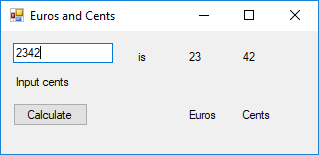
\includegraphics[width=8cm]{var_eurocents}
			\caption{Screenshot of Euros and Cents.}
			\label{fig:var_eurocents}
		\end{figure}


		Some labels will display help for the user, and normally we set their \keyword{Text} property at design-time via the properties window. Their text need not change as the program runs. For labels that will display results, we set their \keyword{Text} property at run-time, as shown above. Text boxes can be overwritten by the user, but labels are protected from being overwritten.
		
		We access properties with the familiar 'dot' notation: recall our use of graphics:
		\begin{lstlisting}
paper.DrawRectangle(myPen, 10, 10, 100, 100)
		\end{lstlisting}
		In general, classes have both methods and properties. Methods make objects do things, whereas properties let us access the current state of an object.
		
		Here is an example program (Euros And Cents) – which breaks down a number of cents into euros and cents. We looked at the use of \ and \keyword{Mod} earlier in this chapter. A screenshot of its execution is shown in \Vref{fig:var_eurocents}. The program uses a text box and several labels.
		\begin{lstlisting}
Private Sub Button1_Click(
		sender As System.Object,
		e As System.EventArgs) Handles Button1.Click
	Dim cents As Integer
	cents = CInt(TextBox1.Text)
	EurosLabel.Text = CStr(cents \ 100)
	CentsLabel.Text = CStr(cents Mod 100)
End Sub
		\end{lstlisting}
		The main controls we use are:
		\begin{itemize}
			\item a button to initiate the conversion;
			\item a text box where the user enters a number of cents;
			\item two labels for the display of the number of dollars and number of cents.
		\end{itemize}
		In addition, there are three labels alongside the input text box and the two output labels, to improve the user's understanding of the form. Their text values are:
		\begin{lstlisting}
Input Cents
Euros
Cents
		\end{lstlisting}
		As we explained in \Cref{ch:visual-studio}, our policy is to rename controls when there is more than one instance of the same type of control on a form. In this program:
		\begin{itemize}
			\item there is one button and one text box, so we can leave these with the name that VB provides;
			\item there are two labels which display results, so we choose to rename them;
			\item the remaining labels have their text set at design-time, and are never manipulated by the program. We can safely leave these unaltered.
		\end{itemize}
		Here is a summary of the main properties.

		\begin{center}
			\begin{tabular}{lll}
				\toprule Control &	Property	 & Setting \\ \midrule
				Button1 & Text & Calculate\\
				TextBox1 & Text & (empty)\\
				EurosLabel & Text & (empty)\\
				CentsLabel & Text & (empty)\\ \bottomrule
			\end{tabular}
		\end{center}
		Remember that renaming should be done as soon as you place a control on the form, before double-clicking to create any event code.
		
		When the program runs, the user enters a number in the text box. Clicking the button causes the calculation to take place, and causes results to be placed in the two labels. However, note that we must convert from strings to numbers and vice versa. Here is an extract:
		\begin{lstlisting}
cents = CInt(TextBox1.Text)
EurosLabel.Text = CStr(cents \ 100)
		\end{lstlisting}
		The program illustrates the use of a text box, and the use of labels to display changing results and unchanging messages.

		\begin{stqb}
			\begin{STQ}
				\item	Both message boxes and labels can be used to display results. What is the main difference?
			\end{STQ}
		\end{stqb}


	\section{The InputBox}	
		\begin{figure}[ht]
			\centering
			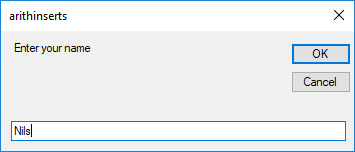
\includegraphics[width=9cm]{var_inputbox}
			\caption{An \keyword{InputBox}}
			\label{fig:var_inputbox}
		\end{figure}
		The input box is rather like a message box, in that it occupies no permanent screen space – it pops up when needed. Like the message box it must be acknowledged, and we can use it to force the user to enter data. You will have encountered this type of input when you log on to a computer. However, the over-use of input boxes can slow down the user interaction. Use them with care. \Vref{fig:var_inputbox} shows the input box created from the first line of code below, where we input a string. The second line shows the input of a number:
		\begin{lstlisting}
Dim n As Integer
Dim s As String
s = InputBox("Enter your name")
n = CInt(InputBox("Enter your age"))
		\end{lstlisting}
		The string in brackets provides a prompt for the user. The input box sends the string that the user enters into our program, where typically we assign it to a variable. In the case of numeric input, we use one of the conversion functions before assigning it. For our introductory programs, we assume that the user will not make a typing error, and will not cancel the input box.
	
	\section{Converting between numbers}
		Sometimes, we need to convert numeric values from one type to another. The most common cases are converting an \keyword{Integer} to a \keyword{Double}, and a \keyword{Double} to an \keyword{Integer}. Here are some examples:
		\begin{lstlisting}
Dim i As Integer = 33
Dim d As Double = 3.9
Dim d1 As Double
d1 = i	' set to 33
' or, explicitly:
d1 = CDbl(i)	' set to 33
i = CInt(d)	' set to 4
		\end{lstlisting}
		The main points are:
		\begin{itemize}
			\item assigning an \keyword{Integer} to a \keyword{Double} works without any additional programming. This is safe, as no information can be lost – there are no decimal places to worry about;
			\item assigning a \keyword{Double} to an \keyword{Integer} requires that something be done with the decimal places, which will not fit into the integer. Because of this potential loss of information, VB requires that we explicitly use type conversion (e.g. by using \keyword{CInt}). The double value is rounded to the nearest integer as it is converted.
		\end{itemize}

		\begin{stqb}
			\begin{STQ}
			\item	What are the values of \keyword{a, b, c, i, j, k} after the following code is executed?
					\begin{lstlisting}
Dim i, j, k As Integer
Dim a, b, c As Double
Dim x As Integer = 3
Dim y As Double = 2.7
i = CInt(y)
j = CInt(y + 0.6)
k = CInt(CDbl(x) + 0.2)
a = x
b = CInt(y)
c = CDbl(y)
					\end{lstlisting}
			\end{STQ}
		\end{stqb}

	\section{The role of expressions}
		Though we have emphasized that expressions (calculations) can form the right-hand side of assignment statements, they can occur in other places. In fact, we can place an \keyword{Integer} expression anywhere we can place a single \keyword{Integer}. Recall our use of the \keyword{DrawLine} method, which has four integers specifying the start and end of the line. We could (if it was useful) replace the numbers with variables, or with expressions:
		\begin{lstlisting}
Dim x As Integer = 100
Dim y As Integer = 200
paper.DrawLine(myPen, 100, 100, 110, 110)
paper.DrawLine(myPen, x, y, x + 50, y + 50)
paper.DrawLine(myPen, x * 2, y – 8, x * 30 – 1, y * 3 + 6)
		\end{lstlisting}
		The expressions are calculated, and the resulting values are passed into DrawLine for it to make use of.
		
	\section{Programming principles}
		\begin{itemize}
			\item A variable has a name, which the programmer chooses.
			\item Variables are declared with \keyword{Dim}.
			\item A variable holds a value.
			\item The value of a variable can be changed with an assignment statement.
		\end{itemize}

	\section{Programming pitfalls}
		\begin{itemize}
			\item Take care with the spelling of variable names. For example, in:
				\begin{lstlisting}
Dim circ1e As Integer ' misspelling
circle = 20
				\end{lstlisting}
				there is a misspelling of a variable, using a '1' (one) instead of a lower-case 'L'. The VB compiler will complain about the second spelling being undeclared. Another favourite error is using a zero instead of a capital 'O'.
			\item Compilation errors are tricky to spot at the beginning. Though the VB compiler gives an indication of where it thinks the error is, the actual error could be in a previous line.
			\item Brackets must balance – there must be the same number of '(' as ')'.
			\item When using numbers with the text property of labels and text boxes, remember to use the string conversion facilities.
			\item When multiplying items, you must place * between them, whereas in maths it is omitted.
		\end{itemize}
	
	\section{Grammar spot}
		\begin{itemize}
			\item Use Dim to declare all variables, as in:
				\begin{lstlisting}
Dim myVariable As Integer
Dim yourVariable As String = "Hello there!"
				\end{lstlisting}
			\item The most useful types are \keyword{Integer}, \keyword{Double}, and \keyword{String}.
			\item The arithmetic operators are \textasciicircum, *, /, \, \keyword{Mod}, +, –.
			\item The \keyword{\&} operator is used to join strings.
			\item We can convert numbers to strings with \keyword{CStr}.
			\item We can convert strings to numbers with \keyword{CInt} and \keyword{CDbl}.
			\item We can obtain a string from the user with an input box, as in:
				\begin{lstlisting}
someString = InputBox("message")
				\end{lstlisting}
		\end{itemize}

	\section{New language elements}
		\begin{itemize}
			\item \keyword{Dim Double Integer String}.
			\item The operators + – * / \ \textasciicircum\ \keyword{Mod} \keyword{\&}.
			\item = for assignment.
			\item Type conversion: \keyword{CStr} \keyword{CInt} \keyword{CDbl}.
		\end{itemize}

	\section{New IDE facilities}
		\begin{itemize}
			\item The \keyword{TextBox} and \keyword{Label} controls, with their \keyword{Text} properties.
			\item The renaming of controls.
			\item The \keyword{InputBox}.
		\end{itemize}

	\section{Summary}
		\begin{itemize}
			\item Variables are used to hold (store) values. They keep their value until explicitly changed (e.g. by another assignment statement).
			\item Operators operate on values.
			\item An expression is a calculation which produces a value. It can be used in a variety of situations, including the right-hand side of an assignment, and as an argument of a method call.
		\end{itemize}

	\section{Exercises}
		\begin{enumChapter}
			\item Extend the rectangle program provided in this chapter to compute the volume of a box, given its three dimensions.
			\item	
				\begin{enumerate}[label=(\alph*)]
					\item Using the following value:
						\begin{lstlisting}
Dim radius As Double = 7.5
						\end{lstlisting}
						use assignment statements to calculate the circumference of a circle, the area of a circle, and the volume of a sphere, based on the same radius. Display the results with messages boxes. The message should state what the result is, rather than merely displaying a number. These calculations involve the use of Pi, which is 3.14 approximately. However, VB provides us with this value to more digits of precision. It is part of the Math class, as the following formulae show its use:
						\begin{lstlisting}
circumference = 2* Math.PI * radius
area = Math.PI * radius ^ 2
volume = (4 / 3) * Math.PI * radius ^ 3
						\end{lstlisting}
					\item Modify part (a) so that the value of the radius is obtained from an input box.
					\item Modify part (a) to use a text box for the input of the radius, and labels for results. Use additional labels to clarify the presentation of the results.
				\end{enumerate}
			\item	Two students take a VB exam, and their results are assigned to two variables:
				\begin{lstlisting}
Dim mark1 As Integer = 44
Dim mark2 As Integer = 51
				\end{lstlisting}
				Write a program which calculates and displays the average mark as a \keyword{Double} value. Check your answer with a calculator.
			\item	Two students take a VB exam, and their results – as produced by a very discriminating examiner – are \keyword{Double} values. Write a program which calculates and displays the average mark as a \keyword{Double} value. Check your answer with a calculator.
			\item	Assume that individuals are taxed at 20\% of their income. Obtain an income value from a text box, then calculate and display the initial amount, the amount after deductions, and the deducted amount. Use labels to make the results understandable.
			\item	Using \keyword{Double} types, write a program which converts a Fahrenheit temperature to its Celsius (centigrade) equivalent. The formula is:
				\begin{lstlisting}
c = (f – 32) * 5 / 9
				\end{lstlisting}
			\item	We are provided with an initial number of seconds:
				\begin{lstlisting}
Dim totalSeconds As Integer = 2549
				\end{lstlisting}
				Write a program to convert this to hours, minutes and seconds. Do an example with pen and paper before you write the program. Use one message box to display the result, is the form:
				\begin{lstlisting}
H:1 M:24 S:9
				\end{lstlisting}
			\item	This problem is to do with electrical resistors, which 'resist' the flow of electrical current through them. An analogy is a hosepipe – a thin one has a high resistance, and a thick one has a low resistance to water. We can imagine connecting two hosepipes in series, resulting in a higher resistance, or in parallel, reducing the resistance (effectively, a fatter pipe). Starting with:
				\begin{lstlisting}
Dim r1 as Double = 4.7
Dim r2 As Double = 6.8
				\end{lstlisting}
				calculate and display the series resistance, given by:
				\begin{align*}
					series = r1 + r2
				\end{align*}
				and the parallel resistance, given by:
				\begin{equation*}
					parallel = \frac{r1 * r2}{r1 + r2}
				\end{equation*}
			\item	We require some software for installation in a British drink-dispensing machine. Here are the details: all items cost less than 1 pound (100 pence), and a 1 pound coin is the highest value that can be inserted. Given the amount inserted and the cost of the item, your program should give change, using the lowest number of coins. For example, if we had:
				\begin{lstlisting}
Dim amountGiven As Integer = 100
Dim itemCost As Integer = 45
				\end{lstlisting}
				the result should be a series of message boxes (one for each coin) of the form:
				\begin{lstlisting}
Number of 50 pence coins is 1
Number of 20 pence coins is 0
Number of 10 pence coins is 0
Number of 5 pence coins is 1
Number of 2 pence coins is 0
Number of 1 penny coins is 0
				\end{lstlisting}
				Hint: work in cents, and make extensive use of the \keyword{Mod} operator. The coin values in pence are: 100, 50, 20, 10, 5, 2, 1.
			\item Write a program which calculates the final amount (f) left in a bank account. The initial amount (i), number of years (n), and compound interest rate (r) per year can vary. Use the formula:
				
				\begin{equation*}
					f = i \left[ 1 + \frac{r}{100} \right]^n
				\end{equation*}
		\end{enumChapter}
		
		\begin{stab}
			\begin{enumChapter}
			\item	\keyword{volume} – allowed, correct style

						\keyword{AREA} – allowed, but area preferred;

						\keyword{Length} – allowed, but lower-case l preferred;

						\keyword{3sides} – not allowed, starts with a digit;

						\keyword{side1} – allowed, correct style;

					\keyword{lenth} – allowed, even with incorrect spelling of length;

					\keyword{mysalary} – allowed, but capital S is preferred;

					\keyword{your salary} – not allowed (no spaces allowed in middle of a name);

					\keyword{screenSize} – allowed, correct style;

					\keyword{Dim} – not allowed – it is a keyword.
				\item	The final values of \keyword{a, b, c, d} are 5, 7, 12, 8.
				\item	Unfortunately, you get zero, as (1 \ 2) is calculated first, resulting in 0. Use / instead.
				\item	The final values of \keyword{a, b, c, d} are 2, 8, 1, 0.333333 etc.
				\item	\begin{lstlisting}
Dim totalSeconds As Integer = 307
Dim seconds, minutes As Integer
minutes = totalSeconds \ 60
seconds = totalSeconds Mod 60
					\end{lstlisting}
				\item	The final values of \keyword{m, n} and \keyword{s} are 334, 37 and 64.
				\item	A label displays its results on the form, and requires no further user interaction. A message box pops up, and the user must click 'OK' to remove it. Thus, the message box forces the user to acknowledge its presence.
				\item	The values of the \keyword{Integer} variables \keyword{i, j, k} are 3, 3, 3, and the values of the \keyword{Double} variables \keyword{a, b, c} are 3.0, 3.0, 2.7.
			\end{enumChapter}
		\end{stab}

